\subsection{Two electrons in two dimensions}

We start with the simple case of two electrons in a harmonic oscillator trap. These electrons do not interact with eachother and the trial wavefunction is given by Eq. \ref{eq:trial_wf_not_interacing}. 

\subsubsection{Brute force sampling}

First, brute force sampling was used to calculate the new position and evaluate the metropolis ratio. The double derivative of the wavefunction, used to calculate the kinetic energy part of the expectation energy, was evaluated both analytically and numerically. Table \ref{tab:brute_force_no_interaction_2p} shows the energy for different values for the parameter $\alpha$. The numbers show that the standard error of the mean (SEM) is underestimating the deviations. From Tab. \ref{tab:brute_force_no_interaction_2p} one can observe that including the correlations, e.g. correlations in the random number generator, increases the deviation, giving us $\sigma_b$. This value is also an estimate of the error, but probably a more true estimate of the error.

From Tab. \ref{tab:brute_force_no_interaction_2p} one can also observe that $\alpha $ = 1.0 gives zero standard deviation and is therefore the optimal parameter. By comparing the results for the analytical and the numerical cases one can observe that the SEM and $\sigma_b$ is similar for both cases, especially around the ground state ($\alpha$ = 1.0). If he expectation energies from the analytial case and the numbercal cases are compared, they differ with values at the scale of $10^{-3}$, which is reasonable with a $\sigma_b$ around $10^{-3}$ to $10^{-2}$. At last one can observe, both from the individual CPU time measurements and the mean CPU time of these 10 measurements (though with different $\alpha$s), that the analytical solution of the double derivative is much faster and more efficient than the numerical case. 

\begin{table}[H]\caption{Comparing the results for analytical/numerical evaluation of the double derivative. Energy are in atomic units (a.u.) and CPU time is in units of seconds. Number of MC cycles are 2$^{21}$.}\label{tab:brute_force_no_interaction_2p}
\center
\begin{tabular}{l|l}
Analytical: &  Numerical:\\ \hline
\begin{tabular}{ccccc}
$\alpha$: & $\left< E_L \right>$: & SEM: & $\sigma_B$: & CPU time:\\ \hline
0.50 & 2.49402 & 0.00073 & 0.01022 & 5.57812\\
0.60 & 2.26441 & 0.00052 & 0.00690 & 5.76562\\
0.70 & 2.13118 & 0.00035 & 0.00448 & 5.92188\\
0.80 & 2.05016 & 0.00022 & 0.00263 & 5.67188\\
0.90 & 2.01015 & 0.00010 & 0.00116 & 5.96875\\
1.00 & 2.00000 & 0.00000 & 0.00000 & 5.62500\\
1.10 & 2.00871 & 0.00009 & 0.00102 & 6.20312\\
1.20 & 2.03402 & 0.00018 & 0.00175 & 6.34375\\
1.30 & 2.07259 & 0.00026 & 0.00244 & 5.95312\\
1.40 & 2.11041 & 0.00034 & 0.00311 & 6.15625\\ \hline
\end{tabular} & \begin{tabular}{ccccc}
$\alpha$: & $\left< E_L \right>$: & SEM: & $\sigma_B$: & CPU time:\\ \hline
0.50 & 2.49991 & 0.00073 & 0.01093 & 18.20310\\
0.60 & 2.26412 & 0.00053 & 0.00727 & 18.21880\\
0.70 & 2.13039 & 0.00036 & 0.00436 & 18.62500\\
0.80 & 2.04993 & 0.00022 & 0.00269 & 18.46880\\
0.90 & 2.01160 & 0.00010 & 0.00118 & 18.46880\\
1.00 & 2.00000 & 0.00000 & 0.00000 & 18.31250\\
1.10 & 2.00825 & 0.00009 & 0.00097 & 18.35940\\
1.20 & 2.03308 & 0.00018 & 0.00170 & 18.31250\\
1.30 & 2.06460 & 0.00026 & 0.00243 & 20.23440\\
1.40 & 2.11803 & 0.00033 & 0.00308 & 19.00000\\ \hline
\end{tabular}\\
Mean CPU time: 5.91875 & Mean CPU time:  18.62033\\
\end{tabular}
\end{table}

\subsubsection{Including importance sampling}

Figure \ref{fig:comparing_sampling} compare the expectation value of the energy and the acceptance rate of brute force sampling and importance sampling. It can be observed from the right part of the figure that the acceptance rate of both methods increase with decreasing step size, but one can also observe that the acceptance is lower for importance sampling than brute force sampling at large step sizes. These observations could indicate that a small step size would be ideal for both methods. 

\begin{figure}[H]
\center
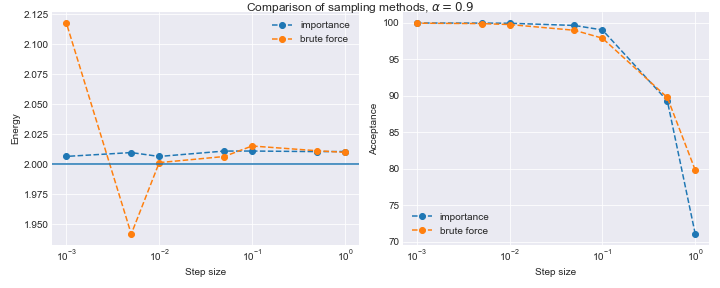
\includegraphics[width=\linewidth]{../Results/comparing_sampling}\caption{Left: Expectation energies after $2^{21}$ MC cycles for different step sizes. Right: Percentage of accepted steps for different step sizes. Here importance sampling and brute force sampling is compared. }\label{fig:comparing_sampling}
\end{figure}


From the left part of the figure it can be observed that one of the expectation values for the energies are lower than the ground state energy ($dl = 0.005$ with brute force sampling) when these calculations where done with $\alpha$ = 0.9. However, in Tab. \ref{tab:importance_no_interaction_2p} which compare the result of brute force sampling and importance sampling for different step sizes one can observe that the standard deviation from the blocking method is larger for the case of brute force sampling with a step size of 0.005. However,  the SEM does not indicate anything to be special about this result.

\begin{table}[H]\caption{Comparing the results for importance/brute force sampling. Energy are in atomic units (a.u.) and CPU time is in units of seconds. Here the parameter $\alpha$ is set to 0.9 and number of MC cycles are 2$^{21}$.}\label{tab:importance_no_interaction_2p}
\begin{tabular}{l|l|l} 
 & Brute force: &  Importance:\\ \hline
\begin{tabular}{c} 
$dl$:\\ \hline
1.000\\
0.500\\
0.100\\
0.050\\
0.010\\
0.005\\
0.001\\
\end{tabular} & \begin{tabular}{ccccc}
 $\left< E_L \right>$: & SEM: & $\sigma_B$: & Acc.: & $t_{CPU}$:\\ \hline
2.010 & 0.00010 & 0.00066 & 79.832& 6.625\\
2.011 & 0.00010 & 0.00112 & 89.794& 7.266\\
2.015 & 0.00011 & 0.00549 & 97.919& 7.078\\
2.007 & 0.00011 & 0.00946 & 99.001& 7.016\\
2.002 & 0.00007 & 0.01510 & 99.788& 6.953\\
1.942 & 0.00006 & 0.02140 & 99.916& 6.578\\
2.118 & 0.00002 & 0.00371 & 99.974& 6.531\\ \hline
\end{tabular} & \begin{tabular}{ccccc}
$\left< E_L \right>$: & SEM: & $\sigma_B$: & Acc.: & $t_{CPU}$:\\ \hline
2.011 & 0.00010 & 0.00022 & 71.078& 8.531\\
2.011 & 0.00010 & 0.00023 & 89.343& 8.672\\
2.011 & 0.00010 & 0.00047 & 99.049& 8.859\\
2.011 & 0.00010 & 0.00068 & 99.662& 8.188\\
2.007 & 0.00010 & 0.00136 & 99.968& 8.281\\
2.010 & 0.00010 & 0.00199 & 99.989& 8.547\\
2.007 & 0.00010 & 0.00410 & 99.999& 8.016\\ \hline
\end{tabular}\\
& Mean CPU time: 6.86384 & Mean CPU time: 8.44197 \\
\end{tabular}
\end{table}

I took a closer look at the actual local energies for the brute force sampling method. Figure \ref{fig:brute_force_small_steps} shows how the energy is not stable for steps sizes smaller than 0.01, so even though the step sizes 0.001 and 0.01 seems to give reasonable expectation values for the energy (see Tab. \ref{tab:importance_no_interaction_2p} and Fig. \ref{fig:comparing_sampling}), Fig. \ref{fig:brute_force_small_steps} seems to show that that is sort of a lucky shot. I also saw this by running the calculation with brute force sampling and the step size, $0.005$, with different seeds for the random number generator. The expectation energy for five different runs where $\left< E_L \right>$ =  1.91487, 2.03452, 1.90805, 1.88356 and 1.9284. From Fig. \ref{fig:brute_force_larger_steps} one can observe that even $dl=0.1$ seems to be too small since it also results in the local energy varying slowly and taking longer "trips" to higher energies and using many steps to get back down again, but for this step size the "trips" to higher energies are more frequent than for the smaller step sizes. I concluded that a step size of 0.5 is the best choice for the brute force sampling because it gives resonable changes of the local energy and an accpentance rate of $\sim$ 90 \% (see Fig. \ref{fig:comparing_sampling}). 

\begin{figure}[H]
\begin{subfigure}{.5\textwidth}
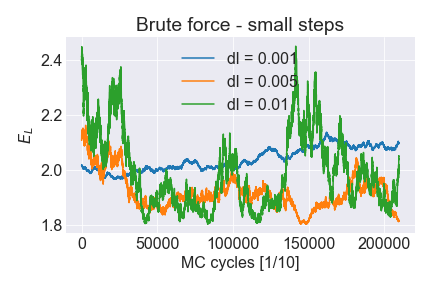
\includegraphics[width=\linewidth]{../Results/brute_force_small_steps}\caption{}\label{fig:brute_force_small_steps}
\end{subfigure}
\begin{subfigure}{.5\textwidth}
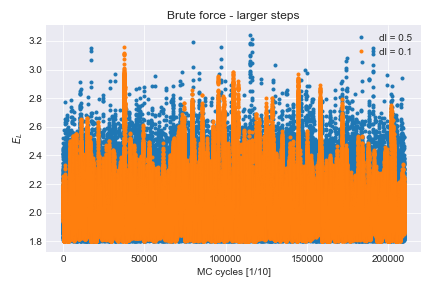
\includegraphics[width=\linewidth]{../Results/brute_force_larger_steps}\caption{}\label{fig:brute_force_larger_steps}
\end{subfigure}
\caption{The local energy for every tenth MC cycle for brute force sampling at different step sizes, $dl$. a) shows the smaller step sizes and b) some that are a bit larger. }\label{fig:brute_force_step_sizes}
\end{figure}

%On the other hand, for the importance sampling, the investigation of the local energies did not give any clues to why the expecation energy is lower that the ground state energy for a step size of 0.5. Eventually I decided that the result itself indicate that 0.5 is a too large step size for importance sampling and taken together with a low acceptance rate at 0.5 ($\sim$ 82 \%) it is clear that a smaller step size is preferable. 
%
%At last, it is interesting to note that the CPU time of importance sampling is higher than the brute force sampling, so even though brute force sampling has a lower acceptance rate, at the ideal step size, than importance sampling the two methods seems to be somewhat comparable at least for the system I am investigating.

Proceeding to evaluate the energy, Table \ref{tab:ground_state_energy_different_omegas_no_interaction_2p} shows how the energy changes with different trap frequencies, $\omega$. In this table one can observe that there is no large difference between the reuslts from brute force sampling and importance sampling. However, to be able to compare the sampling methods more thoroughly it is better to look at the case where the system is not in the ground state. 

\textit{JEG KOM HIT :)}

\begin{table}[H]\caption{Ground state energy of two electrons in harmonic oscillator trap. Number of MC cycles are $2^{23}$.}\label{tab:ground_state_energy_different_omegas_no_interaction_2p}
\begin{tabular}{l|l|l} 
 & Brute force: &  Importance:\\ \hline
\begin{tabular}{c} 
$\omega$  \\ \hline
1.00  \\
0.50  \\
0.10  \\
0.05  \\
0.01  \\
\end{tabular} & \begin{tabular}{ccccc}
$\alpha$ & $\left< E_L \right>$ & $\overline{r}_{12} $ & $\left< T \right>$  & $\left< V_{ext}\right>$ \\ \hline
1 & 2.00 & 1.250 & 1.0008 & 0.9992\\
1 & 1.00 & 1.775 & 0.4971 & 0.5029\\
1 & 0.20 & 3.967 & 0.0996 & 0.1004\\ 
1 & 0.10 & 5.638 & 0.0497 & 0.0503\\ 
1 & 0.02 & 12.631 & 0.0099 & 0.0101\\  
\end{tabular} & \begin{tabular}{ccccc}
$\alpha$ & $\left< E_L \right>$ & $\overline{r}_{12} $ & $\left< T \right>$  & $\left< V_{ext}\right>$ \\ \hline
1 & 2.00 & 1.254 & 0.9982 & 1.0018\\
1 & 1.00 & 1.781 & 0.4973 & 0.5027\\
1 & 0.20 & 4.046 & 0.0987 & 0.1013\\ 
1 & 0.10 & 5.534 & 0.0512 & 0.0488\\ 
1 & 0.02 & 12.488 & 0.0101 & 0.0099\\ 
\end{tabular}\\
\end{tabular}
\end{table}

\begin{table}[H]\caption{Comparing the results for brute force sampling/importance sampling. Energy are in atomic units (a.u.) and CPU time is in units of seconds. Number of MC cycles are 2$^{21}$.}\label{tab:compare_importance_alphas_2p}
\center
\begin{tabular}{l|l|l}
 & Brute force: & Importance:\\ \hline
\begin{tabular}{c}
$\alpha$: \\ \hline
0.50 \\
0.60 \\
0.70 \\
0.80 \\
0.90\\
1.00 \\
1.10 \\
1.20 \\
1.30\\
1.40 \\ \hline
\end{tabular} & \begin{tabular}{cccc}
 $\left< E_L \right>$: & SEM: & $\sigma_B$: & CPU time:\\ \hline
2.49074 & 0.00072 & 0.01030 & 6.26562\\
2.27645 & 0.00053 & 0.00721 & 6.53125\\
2.12481 & 0.00036 & 0.00451 & 6.59375\\
2.04873 & 0.00022 & 0.00265 & 6.68750\\
2.01135 & 0.00010 & 0.00115 & 6.82812\\
2.00000 & 0.00000 & 0.00000 & 6.75000\\
2.00863 & 0.00009 & 0.00097 & 6.59375\\
2.03343 & 0.00018 & 0.00174 & 7.29688\\
2.07103 & 0.00026 & 0.00246 & 6.75000\\
2.11725 & 0.00033 & 0.00317 & 6.70312\\ \hline
\end{tabular} & \begin{tabular}{cccc}
$\left< E_L \right>$: & SEM: & $\sigma_B$: & CPU time:\\ \hline
2.52950 & 0.00075 & 0.01952 & 8.53125\\
2.26531 & 0.00052 & 0.01281 & 8.62500\\
2.12449 & 0.00036 & 0.00813 & 8.76562\\
2.04797 & 0.00022 & 0.00454 & 9.37500\\
2.01171 & 0.00010 & 0.00203 & 8.81250\\
2.00000 & 0.00000 & 0.00000 & 8.76562\\
2.00954 & 0.00009 & 0.00171 & 8.40625\\
2.03276 & 0.00018 & 0.00305 & 8.50000\\
2.07363 & 0.00026 & 0.00440 & 8.67188\\
2.10697 & 0.00034 & 0.00536 & 8.67188\\ \hline
\end{tabular}\\
& Mean CPU time:  6.7000 & Mean CPU time:  8.7125\\
\end{tabular}
\end{table}

\subsubsection{Including optimization}

Minimization rate of 0.5 seemed to be ideal. It resulted in the fewest steps until the parameter value stabilized both for guesses close to the optimal value and for guesses far away from the optimal value, but for the smallest trap frequencies I had to use $\gamma = $ 0.1 or 0.2. The parameters were optimized by trying out different first guesses for $\alpha$ and $\beta$ and tuning $\gamma$ so that the parameters stabilized during the first 200 iteretions. The optimal parameters were extracted from the mean of the last 50 iterations. An example run is shown in Fig. \ref{} for $\omega = 0.5$.

\subsubsection{Including interaction}

\begin{table}[H]\caption{Ground state energy of two interacting electrons in harmonic oscillator trap found with brute force sampling. Number of MC cycles are $2^{23}$}\label{tab:ground_state_energy_brute_force_interaction}
\center
\begin{tabular}{c|cccccrccc}
$\omega$ & $\alpha$ & $\beta$ & $\left< E_L \right>$ & SEM & $\sigma_B$ &  $\overline{r}_{12} \,\,\,$ & $\left< T \right>$  & $\left< V_{ext}\right>$ & $\left<V_{int} \right>$  \\ \hline
1.00 & 0.98847 & 0.39965 & 3.0068 & 0.00001 & 0.00009 & 1.636 & 0.8944 & 1.2990 & 0.8135\\
0.50 & 0.98061 & 0.31091 & 1.6674 & 0.00001 & 0.00010 & 2.481 & 0.4488 & 0.7051 & 0.5135\\
0.10 & 0.94693 & 0.17764 & 0.4486 & 0.00001 & 0.00011 & 6.695 & 0.1003 & 0.1767 & 0.1716\\
0.05 & 0.92747 & 0.13815 & 0.2609 & 0.00000 & 0.00011 & 10.389 & 0.0533 & 0.0997 & 0.1076\\
0.01 & 0.88398 & 0.07287 & 0.0777 & 0.00000 & 0.00006 & 29.177 & 0.0129 & 0.0284 & 0.0364\\
\end{tabular}
\end{table}

\begin{table}[H]\caption{Ground state energy of two interacting electrons in harmonic oscillator trap found with importance sampling. Number of MC cycles are $2^{23}$}\label{tab:ground_state_energy_importance_interaction}
\center
\begin{tabular}{c|ccccccccc}
$\omega$ & $\alpha$ & $\beta$ & $\left< E_L \right>$ & SEM & $\sigma_B$ &  $\overline{r}_{12} \,\,\,$ & $\left< T \right>$  & $\left< V_{ext}\right>$ & $\left<V_{int} \right>$  \\ \hline
1.00 & 0.98846 & 0.39954 & 3.0069 & 0.00001 & 0.00018 & 1.643 & 0.8931 & 1.3052 & 0.8086\\
0.50& 0.98082 & 0.31068 & 1.6674 & 0.00001 & 0.00019 & 2.481 & 0.4547 & 0.6997 & 0.5130\\
0.10 & 0.94734 & 0.17810 & 0.4486 & 0.00001 & 0.00023 & 6.724 & 0.0989 & 0.1787 & 0.1710\\
0.05 & 0.92262 & 0.14090 & 0.2610 & 0.00000 & 0.00021 & 10.333 & 0.0495 & 0.1024 & 0.1091\\
\end{tabular}
\end{table}

\subsection{One-body density}

\begin{figure}[H]
\center
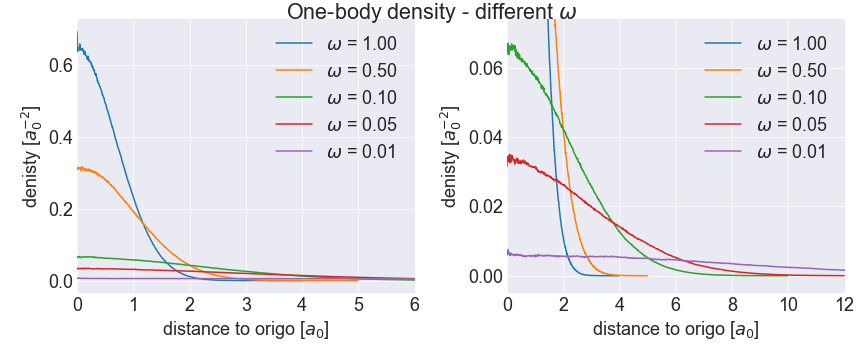
\includegraphics[width=0.8\linewidth]{../Results/one_body_density_no_interaction_2p}\caption{•}\label{fig:one_body_density_no_interaction_2p}
\end{figure}

\begin{figure}[H]
\center
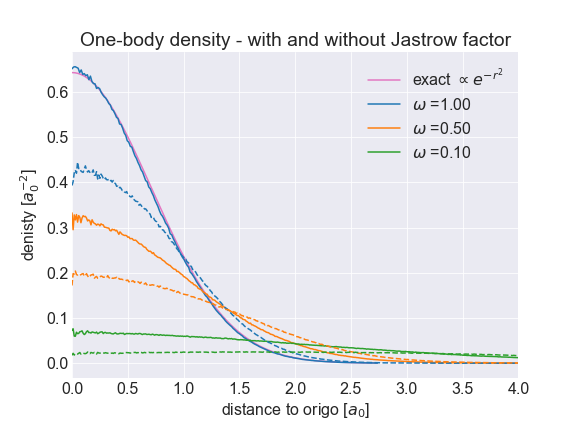
\includegraphics[width=0.7\linewidth]{../Results/one_body_density_interaction_2p}\caption{Dashed lines are with the Jastrow factor. Normal lines is without Jastrow factor. }\label{fig:one_body_density_interaction_2p}
\end{figure}

\subsection{Extending to more particles}

\subsubsection{Six particles}

\begin{table}[H]\caption{Number of MC cycles are $2^{23}$. }\label{tab:ground_state_energy_importance_6p}
\center
\begin{tabular}{c|rcc}
$\omega$ & $\left< E_L \right>$  & $\left< T \right>$  & $\left< V_{ext}\right>$ \\ \hline
1.00 & 10.00 & 4.9865 & 5.0135\\ 
0.50 & 5.00 & 2.4973 & 2.5027\\
0.10 & 1.00 & 0.4861 & 0.5139\\
0.05 & 0.50 & 0.2483 & 0.2517\\
0.01 & 0.10 & 0.0454 & 0.0546\\
\end{tabular}
\end{table}

\begin{table}[H]\caption{Ground state energy of two interacting electrons in harmonic oscillator trap found with importance sampling. Number of MC cycles are $2^{23}$}\label{tab:ground_state_energy_importance_interaction_6p}
\center
\begin{tabular}{c|cccccccc}
$\omega$ & $\alpha$ & $\beta$ & $\left< E_L \right>$ & SEM & $\sigma_B$ &  $\left< T \right>$  & $\left< V_{ext}\right>$ & $\left<V_{int} \right>$  \\ \hline
1.00 & 0.71567 & 0.49372 & 20.4492 & 0.00022 & 0.00813 & 2.3429 & 10.7076 & 7.3988\\
0.50 & 0.75823 & 0.34260 & 11.9868 & 0.00011 & 0.00522 & 1.3226 & 5.8094 & 4.8548\\
0.10 & 0.78852 & 0.15041 & 3.6542 & 0.00003 & 0.00416 & 0.2951 & 1.7035 & 1.6556\\
0.05 & 0.76518 & 0.10733 & 2.2223 & 0.00003 & 0.00436 &  0.1178 & 1.0882 & 1.0162\\
\end{tabular}
\end{table}

\begin{figure}[H]
\center
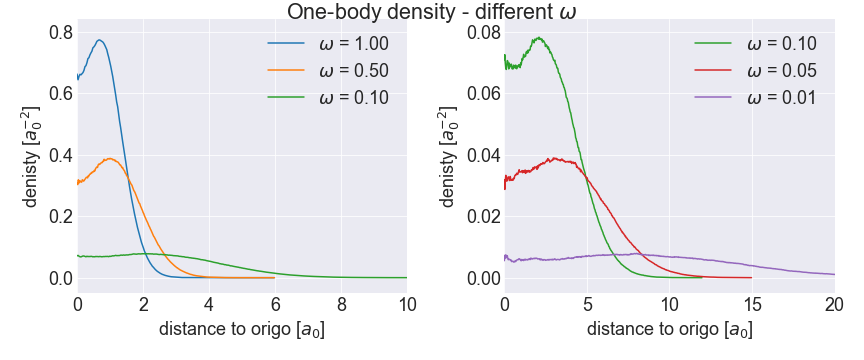
\includegraphics[width=0.8\linewidth]{../Results/one_body_density_no_interaction_6p}\caption{•}\label{fig:one_body_density_no_interaction_6p}
\end{figure}

\begin{figure}[H]
\center
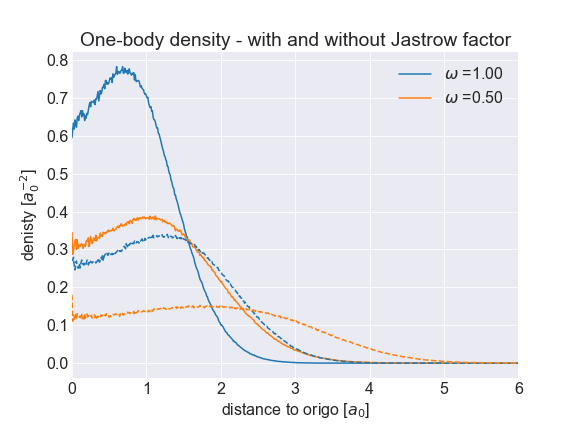
\includegraphics[width=0.7\linewidth]{../Results/one_body_density_interaction_6p}\caption{Dashed lines are with the Jastrow factor. Normal lines is without Jastrow factor. }\label{fig:one_body_density_interaction_6p}
\end{figure}


\subsubsection{Twelve particles}

\begin{table}[H]\caption{Number of MC cycles are $2^{23}$. }\label{tab:ground_state_energy_importance_12p}
\center
\begin{tabular}{c|rrr}
$\omega$ & $\left< E_L \right>$  & $\left< T \right>\,\,\,$  & $\left< V_{ext}\right>\,$ \\ \hline
1.00 & 28.00 & 14.0117 & 13.9883\\ 
0.50 & 14.00 & 7.0463 & 6.9537\\ 
0.10 & 2.80 & 1.4084 & 1.3916\\ 
0.05 & 1.40 & 0.6901 & 0.7099\\ 
0.01 & 0.28 & 0.1419 & 0.1381\\ 
\end{tabular}
\end{table}

\begin{figure}[H]
\center
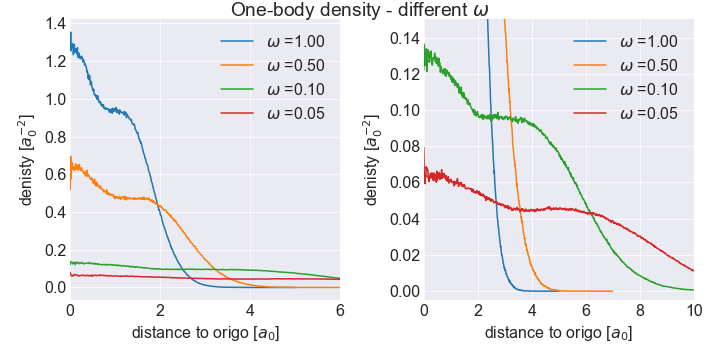
\includegraphics[width=0.8\linewidth]{../Results/one_body_density_no_interaction_12p}\caption{Had to use MC 2 24 to get smooth graphs. }\label{fig:one_body_density_no_interaction_12p}
\end{figure}